\section{Cloud Architektur}

Bei den Cloud Architekturen gibt es genau 3 verschiedene Rollen:
\begin{enumerate}
	\item \textbf{Provider:} bietet Cloud Produkte/Lösungen an
	\item \textbf{Konsumenten:} konsumieren Cloud Lösungen
	\item \textbf{Klient:} nehmen Cloud Lösungen
	 (Anwendungen/Daten) in Anspruch
\end{enumerate}

\subsection{Konzeptuelle Sichtweise}

In diesem Abschnitt werden die Architekturen der einzelnen Kategorien von Cloudlösungen beschrieben.

\subsubsection{Konsumenten Sichtweise}

Wie in \textbf{Abbildung \ref{ConsumerView}} zu sehen, werden Ressourcen in Form von Clustersystemen vom Provider zur Verfügung gestellt.
Einzelne Klienten können über eine Netzwerkverbindung auf diese Ressourcen zeitgleich zugreifen. Der Provider kann außerdem den Pool
von Hardware Ressourcen verwalten, d.h. einzelne Hardware kann stillgelegt und ersetzt werden. Die Klienten werden nach dem stilllegen
auf andere Hardware Ressourcen weitergeleitet.
\todo{eventuell Rest hinzufügen}
\begin{figure}[H]
    \centering
	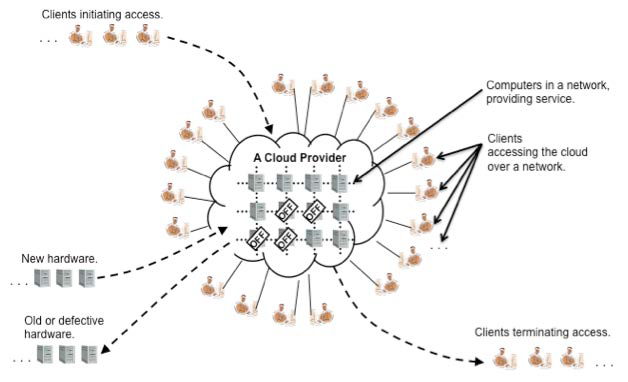
\includegraphics[width=0.4\textwidth]{Images/ConsumerView}
	\caption{Konsumenten Sichtweise \cite{Badger}}
	\label{ConsumerView}
\end{figure}


Alle Kategorien von Cloud-Computing können sogenannte Sicherheitsperimeter verwenden. Diese Regeln den Zugriff auf die Ressource.
In unseren Beispielen kann ein Klient, der sich außerhalb des Sicherheitsperimeter befindet, nur durch einen \glqq boundary controller\grqq
Zugriff zum Netzwerk erlangen.

\subsubsection{Lokale Private Cloud}

Wie in \textbf{Abbildung \ref{PrivateCloud}} zu sehen, befindet sich eine Private Cloud innerhalb der Organisation.
Klienten, die sich innerhalb des Sicherheitsperimeters befinden, können sich mit der Privaten Cloud verbinden. 
Klienten von außerhalb, können eine Verbindung durch den \glqq boundary controller\grqq aufbauen. Dieser Sicherheitsperimeter ist in diesem
Fall optional und wird von dem Konsumenten verwaltet.

\begin{figure}[H]
    \centering
	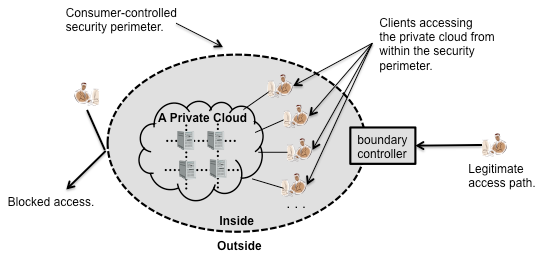
\includegraphics[width=0.4\textwidth]{Images/On-sitePrivateCloud}
	\caption{Private Cloud \cite{Badger}}
	\label{PrivateCloud}
\end{figure}

Die Verwaltung der Cloud wird vom Konsumenten übernommen. Dieser muss die Cloud so einstellen, dass die Arbeitslast zwischen verschiedenen
Maschinen verteilt werden kann, um die Ressourcen optimal nutzen zu können. Außerdem sollten redundante Kopien der Daten auf verschiedenen Maschinen 
gespeichert werden. Dies hat den Vorteil, dass bei einem Serverausfall der Klient auf eine andere Maschine weitergeleitet werden kann.
Außerdem muss der Konsument sicherstellen, dass wichtige Daten wie z.B. Lohnabrechnungen nicht von allen Klienten zugegriffen werden können,
da verschiedenen Daten auf einer Maschine verarbeitet werden können. Der Nachteil von Privaten Clouds ist, dass es hohe Anschaffungskosten, wie z.B. 
das Anschaffen von neuen Daten Zentren, gibt. Außerdem müssen bei z.B. steigenden Zugriffszahlen, neue Hardware vom Konsumenten bereitgestellt werden. 
Dies verringert Flexibilität des Konsumenten.

\subsubsection{Ausgelagerte Private Cloud}

Bei der ausgelagerten Privaten Cloud, wird die Cloud zu einem Provider verlagert. Dieser separiert das Organisationsnetzwerk
von seinem \glqq öffentlichen\grqq Netzwerk, wie in \textbf{Abbildung \ref{OutSourcedPrivateCloud}} zu sehen ist. Das Netzwerk wird vom Provider
durch einen Sicherheitsperimeter geschützt. Der Provider muss dabei sicherstellen, dass die Sicherheitsanforderungen des Konsumenten erfüllt werden. 
Der Konsument kann ebenfalls einen Sicherheitsperimeter in seiner Organisation installieren, um den Zugriff zur Cloud zu regeln.
Die beiden Perimeter werden dann durch einen Kommunikationskanal verbunden und Klienten können dann nur über diesen Kanal auf Daten der Cloud zugreifen.

\begin{figure}[H]
    \centering
	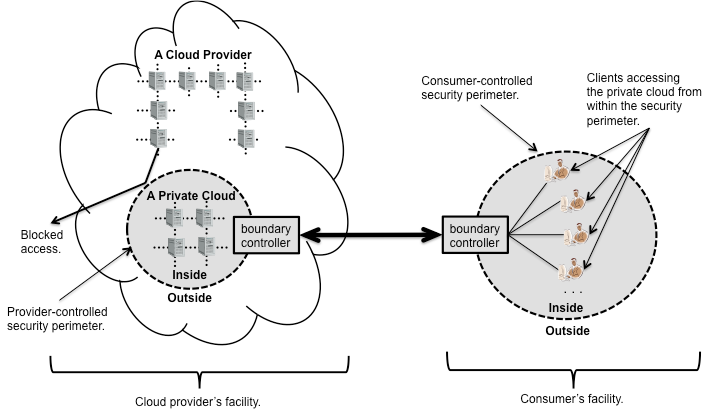
\includegraphics[width=0.4\textwidth]{Images/OutSourcedPrivateCloud}
	\caption{Ausgelagerte Private Cloud \cite{Badger}}
	\label{OutSourcedPrivateCloud}
\end{figure}

Der Konsument ist in diesem Fall von der Netzwerkverfügbarkeit und -geschwindigkeit des Providers abhängig, kann die Geschwindigkeit aber durch Sondertarife erhöhen.
Der Provider muss außerdem sicherstellen, dass die Arbeitslast auf den verschiedenen Maschinen innerhalb des Perimeters verteilt wird und sich die Daten 
nicht mit den Daten von anderen Organisationen, außerhalb des Perimeters, vermischen.
Der Vorteil dieser Architektur ist es, dass der Konsument keine eigenen Ressourcen mehr anschaffen muss und diese beim Provider mieten kann.
Eine Erhöhung der verfügbaren Ressourcen kann jedoch vom Provider nur manuell geschehen, sofern dieser über genug Ressourcen verfügt. 



\subsubsection{Lokale Community Cloud}
abcdeffg
\begin{figure}[H]
    \centering
	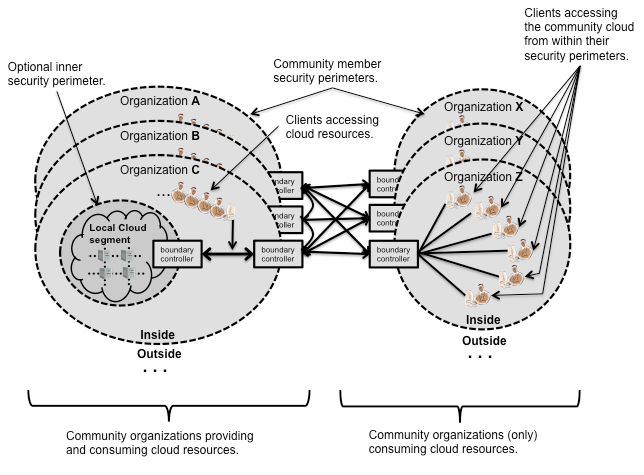
\includegraphics[width=0.4\textwidth]{Images/On-siteCommunityCloud}
	\caption{Lokale Community Cloud \cite{Badger}}
	\label{On-siteCommunityCloud}
\end{figure}



\subsubsection{Ausgelagerte Community Cloud}
\begin{figure}[H]
    \centering
	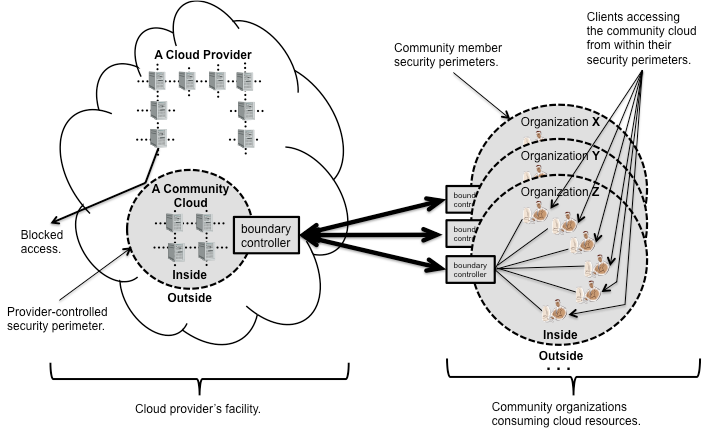
\includegraphics[width=0.4\textwidth]{Images/OutSourcedCommunityCloud}
	\caption{Ausgelagerte Community Cloud \cite{Badger}}
	\label{OutSourcedCommunityCloud}
\end{figure}


\subsubsection{Public Cloud}
\begin{figure}[H]
    \centering
	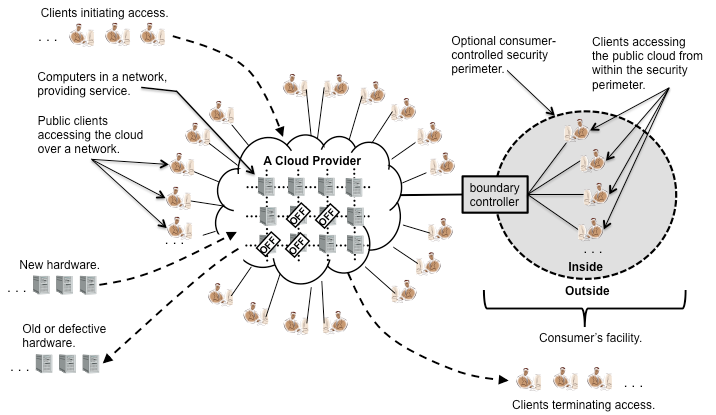
\includegraphics[width=0.4\textwidth]{Images/PublicCloud}
	\caption{Public Cloud \cite{Badger}}
	\label{PublicCloud}
\end{figure}


\subsubsection{Hybrid Cloud}
\begin{figure}[H]
    \centering
	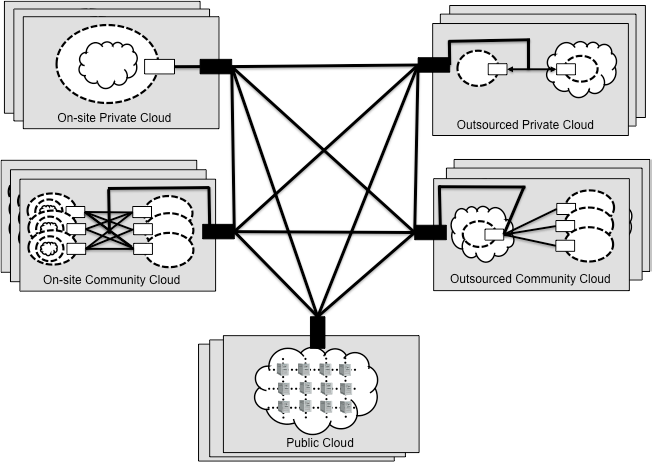
\includegraphics[width=0.4\textwidth]{Images/HybridCloud}
	\caption{Hybrid Cloud \cite{Badger}}
	\label{HybridCloud}
\end{figure}


\subsubsection{SaaS}
\begin{figure}[H]
    \centering
	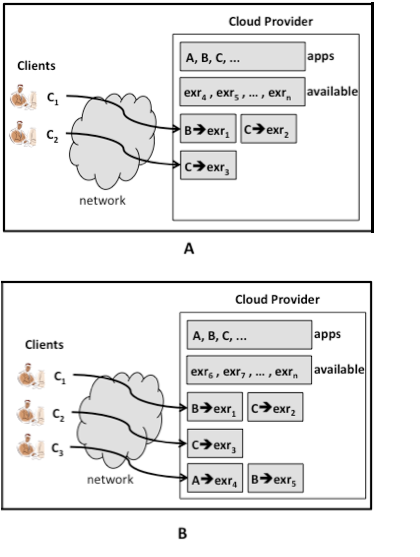
\includegraphics[width=0.4\textwidth]{Images/SaaSInteraction}
	\caption{Hybrid Cloud \cite{Badger}}
	\label{SaaSInteraction}
\end{figure}

\begin{figure}[H]
    \centering
	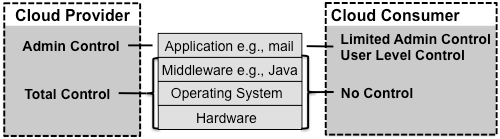
\includegraphics[width=0.4\textwidth]{Images/SaaSControl}
	\caption{Hybrid Cloud \cite{Badger}}
	\label{SaaSControl}
\end{figure}


\begin{figure}[H]
    \centering
	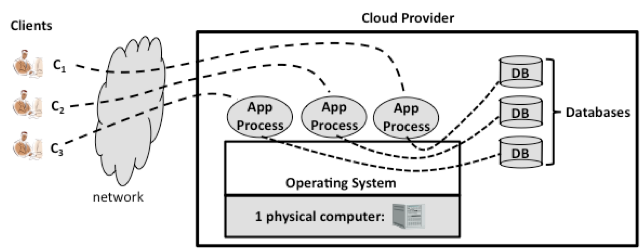
\includegraphics[width=0.4\textwidth]{Images/SaaSM1}
	\caption{Hybrid Cloud \cite{Badger}}
	\label{SaaSM1}
\end{figure}

\begin{figure}[H]
    \centering
	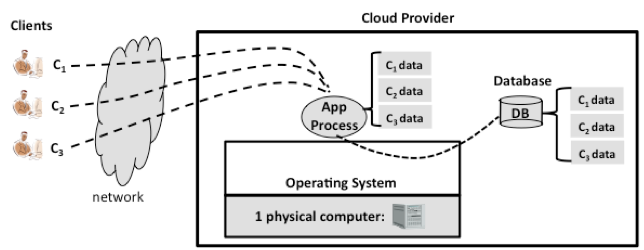
\includegraphics[width=0.4\textwidth]{Images/SaaSM2}
	\caption{Hybrid Cloud \cite{Badger}}
	\label{SaaSM2}
\end{figure}

\subsubsection{Paas}
\begin{figure}[H]
    \centering
	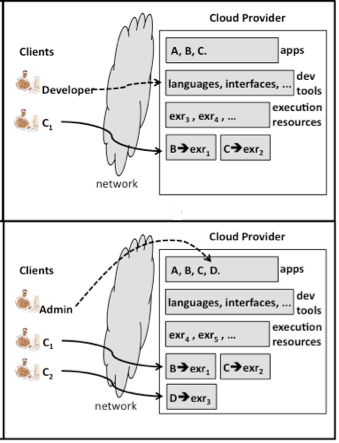
\includegraphics[width=0.4\textwidth]{Images/PaaSInteraction}
	\caption{Hybrid Cloud \cite{Badger}}
	\label{PaaSInteration}
\end{figure}

\begin{figure}[H]
    \centering
	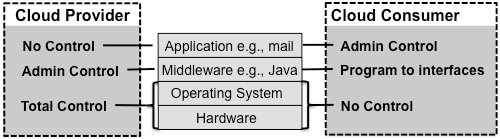
\includegraphics[width=0.4\textwidth]{Images/PaaSControl}
	\caption{Hybrid Cloud \cite{Badger}}
	\label{PaaSControl}
\end{figure}

\subsubsection{IaaS}
\begin{figure}[H]
    \centering
	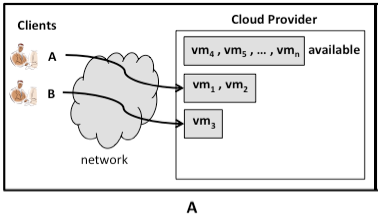
\includegraphics[width=0.4\textwidth]{Images/IaaSInteraction}
	\caption{Hybrid Cloud \cite{Badger}}
	\label{IaaSInteraction}
\end{figure}

\begin{figure}[H]
    \centering
	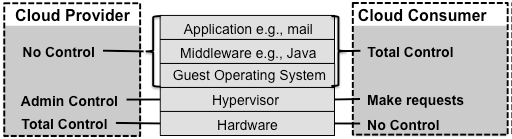
\includegraphics[width=0.4\textwidth]{Images/IaaSControl}
	\caption{Hybrid Cloud \cite{Badger}}
	\label{IaaSControl}
\end{figure}

\subsection{Logische Sichtweise}
\begin{figure}[H]
    \centering
	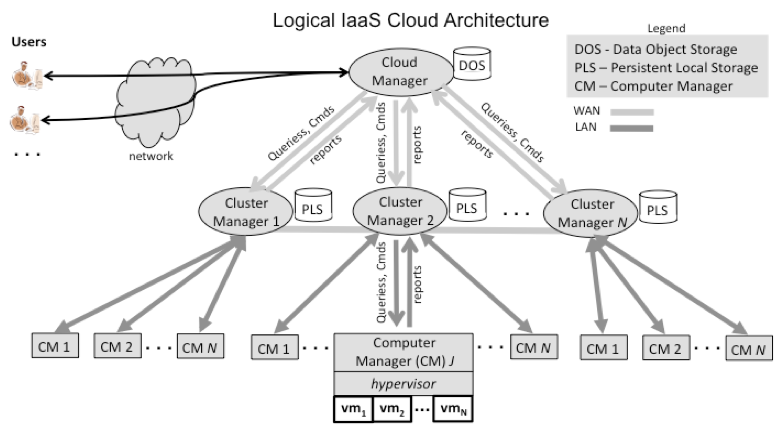
\includegraphics[width=0.4\textwidth]{Images/IaaSLogic}
	\caption{Hybrid Cloud \cite{Badger}}
	\label{IaaSLogic}
\end{figure}

% \subsection{Management}
\pagebreak